\documentclass{article}
\usepackage[utf8]{inputenc}
\usepackage[italian]{babel}
\usepackage{natbib}
\usepackage{graphicx}
\usepackage[table,xcdraw]{xcolor}
\usepackage{listings}
\usepackage{amsmath}
\usepackage{minted}
\usepackage{amsthm}
\usepackage{enumitem}
\usepackage{color}
\usepackage{svg}
\usepackage{pgfplots}
\usepackage[hidelinks]{hyperref}

% ----- NEW SYMBOLS

\newcommand{\imgtick}{\ensuremath{%
  \mathchoice{\includegraphics[height=2ex]{images/symbols/tick.png}}
    {\includegraphics[height=2ex]{images/symbols/tick.png}}
    {\includegraphics[height=1.5ex]{images/symbols/tick.png}}
    {\includegraphics[height=1ex]{images/symbols/tick.png}}
}}

\newcommand{\imgminus}{\ensuremath{%
  \mathchoice{\includegraphics[height=2ex]{images/symbols/minus.png}}
    {\includegraphics[height=2ex]{images/symbols/minus.png}}
    {\includegraphics[height=1.5ex]{images/symbols/minus.png}}
    {\includegraphics[height=1ex]{images/symbols/minus.png}}
}}

\newcommand{\imgplus}{\ensuremath{%
  \mathchoice{\includegraphics[height=2ex]{images/symbols/plus.png}}
    {\includegraphics[height=2ex]{images/symbols/plus.png}}
    {\includegraphics[height=1.5ex]{images/symbols/plus.png}}
    {\includegraphics[height=1ex]{images/symbols/plus.png}}
}}

\newcommand{\imgx}{\ensuremath{%
  \mathchoice{\includegraphics[height=2ex]{images/symbols/x.png}}
    {\includegraphics[height=2ex]{images/symbols/x.png}}
    {\includegraphics[height=1.5ex]{images/symbols/x.png}}
    {\includegraphics[height=1ex]{images/symbols/x.png}}
}}

\newcommand{\imgdivided}{\ensuremath{%
  \mathchoice{\includegraphics[height=2ex]{images/symbols/divided.png}}
    {\includegraphics[height=2ex]{images/symbols/divided.png}}
    {\includegraphics[height=1.5ex]{images/symbols/divided.png}}
    {\includegraphics[height=1ex]{images/symbols/divided.png}}
}}

\newcommand{\imgchina}{\ensuremath{%
  \mathchoice{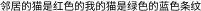
\includegraphics[height=2ex]{images/cinese_esempio.png}}
    {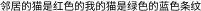
\includegraphics[height=2ex]{images/cinese_esempio.png}}
    {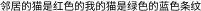
\includegraphics[height=1.5ex]{images/cinese_esempio.png}}
    {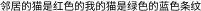
\includegraphics[height=1ex]{images/cinese_esempio.png}}
}}

\newcommand{\imgchinasplitted}{\ensuremath{%
  \mathchoice{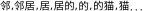
\includegraphics[height=2ex]{images/cinese_esempio_splitted.png}}
    {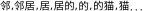
\includegraphics[height=2ex]{images/cinese_esempio_splitted.png}}
    {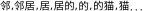
\includegraphics[height=1.5ex]{images/cinese_esempio_splitted.png}}
    {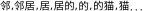
\includegraphics[height=1ex]{images/cinese_esempio_splitted.png}}
}}
\newcommand{\commonCrawlFilesTable}[0]{
    \renewcommand\arraystretch{1.2}
    % Please add the following required packages to your document preamble:
    % \usepackage{graphicx}
    % \usepackage[table,xcdraw]{xcolor}
    % If you use beamer only pass "xcolor=table" option, i.e. \documentclass[xcolor=table]{beamer}
    \begin{table}[h]
    \resizebox{\textwidth}{!}{%
    \begin{tabular}{lllr}
    \rowcolor[HTML]{C0C0C0} 
    Tipo File                                                          & Descrizione                                                                                                                                              & \#Files & \begin{tabular}[c]{@{}r@{}}Dim.dei file\\ compressi\end{tabular} \\ \hline
    \rowcolor[HTML]{EFEFEF} 
    Segments                                                           &                                                                                                                                                          & 100     &                                                                   \\
    WARC files                                                         & Dati grezzi generati dal Crawler                                                                                                                         & 64000   & 59.86 TiB                                                         \\
    \rowcolor[HTML]{EFEFEF} 
    WAT files                                                          & \begin{tabular}[c]{@{}l@{}}Contengono meta-dati relativi ai record nei \\ file WARC\end{tabular}                                                          & 64000   & 18.23 TiB                                                         \\
    WET files                                                          & \begin{tabular}[c]{@{}l@{}}Contengono solo testo semplice estratto \\ dai WARC\end{tabular}                                                              & 64000   & 7.62 TiB                                                          \\
    \rowcolor[HTML]{EFEFEF} 
    Robots.txt files                                                   & \begin{tabular}[c]{@{}l@{}}Files Robot.txt richiesti ai vari siti analizzati \\ (consentono al Crawler di scansionare \\ meglio i siti web)\end{tabular} & 64000   & 170 GiB                                                          \\
    \begin{tabular}[c]{@{}l@{}}Non-200 \\ responses files\end{tabular} & \begin{tabular}[c]{@{}l@{}}Risposte del server con HTTP status code \\ diverso da 200 (404, redirects, ecc.)\end{tabular}                                & 64000   & 1.79 TiB                                                          \\
    \rowcolor[HTML]{EFEFEF} 
    URL index files                                                    & \begin{tabular}[c]{@{}l@{}}Indice degli url analizzati, completo di utili \\ informazioni aggiuntive\end{tabular}                                        & 302     & 210 GiB                                                         
    \end{tabular}%
    }
    \end{table}
    \renewcommand\arraystretch{1.0}
}

%TOTALE: 88791
%tick: 49668
%x: 5371
%plus: 14058
%minus: 14941
%divided: 4753
\newcommand{\printHistogram}[0]{
    %\pgfplotsset{scaled y ticks=false}
    \begin{tikzpicture}
    \begin{axis}[
        symbolic x coords={\imgtick{},\imgx{},\imgplus{},\imgminus{},\imgdivided{}}, 
        ylabel = {occorrenze ($\cdot 10^3$)}, 
        xlabel = {Accuratezza dei risultati}, 
        xtick=data]
        
        \addplot[ybar,fill=white] coordinates {
            (\imgtick{}, 49.668)
            (\imgx{}, 5.371)
            (\imgplus{}, 14.058)
            (\imgminus{}, 14.941)
            (\imgdivided{}, 4.753)
        };
    \end{axis}
    \end{tikzpicture}
}

\newcommand{\printTimeGraph}[0]{
    \begin{tikzpicture}
    \begin{axis}[
      %ymin=20,
      %ymax=90,
      %width=15cm,
      %height=7cm,
      ylabel={tempo (minuti)},
      xlabel={\#files WET analizzati},
      %xticklabels={,2,4,6,8,10}, 
      legend style={at={(0.13,0.83)},
      anchor=west, legend columns=-1, font=\small},
      legend cell align=left,
      xtick=data
     ]

    \addlegendentry{abc}

    \addplot[blue, mark=+] coordinates {
        (2, 1.23)
        (4, 2.32)
        (6, 3.23)
        (8, 4.32)
        (10, 5.45)
    };
    
    \addplot[gray, mark=] coordinates {
        (2, 1.23)
        (4, 2.46)
        (6, 3.69)
        (8, 4.92)
        (10, 6.15)
    };
    \end{axis}
    \end{tikzpicture}
}

\setlist[itemize,1]{label=$\--$}

% ------------------- COMMANDS
\newcommand{\MR}{MapReduce}
%\newcommand{\MRA}{MR Lang Analyzer}
\newcommand{\cld}{\textit{CLD}2}
\newcommand{\WET}{\textit{WET}}
\newcommand{\info}{\textit{info}}
\newcommand{\CC}{Common Crawl}
\newcommand{\isoOne}{ISO 639-1}
\newcommand{\isoTwo}{ISO 639-1}
\newcommand{\pt}{\textit{plain text}}
\newcommand{\filename}[1]{\textit{#1}}
\newcommand{\function}[1]{\textit{#1}}
\newcommand{\command}[1]{\texttt{#1}}
%\newcommand{\mintedstyle}[1]{{\fontfamily{cmvtt}\selectfont #1}}
%\newcommand{\path}[1]{\textit{#1}} #already defined

% ------------------- ENVIROMENTS AND THEOREMS
\newtheorem*{definition}{Definizione}

\title{Analisi della lingua di pagine web\\
            tramite un algoritmo \MR \\ \vskip 5px
            \large Progetto Finale Big Data}
\author{Crosara Marco VR434403}
\date{Marzo 2019 / Aprile 2019}

\begin{document}

\maketitle
\thispagestyle{empty}

\vspace{\fill}

\begin{center}
  UNIVERSITÀ DEGLI STUDI DI VERONA\\
Anno Accademico 2018/2019
\end{center}

\newpage

%Indice
\tableofcontents
\thispagestyle{empty}

\newpage

%\addtocounter{section}{-1}

%  _____ _   _ _______ _____   ____  _____  _    _ ___________ ____  _   _ ______ 
% |_   _| \ | |__   __|  __ \ / __ \|  __ \| |  | |___  /_   _/ __ \| \ | |  ____|
%   | | |  \| |  | |  | |__) | |  | | |  | | |  | |  / /  | || |  | |  \| | |__   
%   | | | . ` |  | |  |  _  /| |  | | |  | | |  | | / /   | || |  | | . ` |  __|  
%  _| |_| |\  |  | |  | | \ \| |__| | |__| | |__| |/ /__ _| || |__| | |\  | |____ 
% |_____|_| \_|  |_|  |_|  \_\\____/|_____/ \____//_____|_____\____/|_| \_|______|

\section{Introduzione}

Il progetto è partito dalla curiosità di analizzare un grosso quantitativo di pagine web con lo scopo di farne in qualche modo categorizzazione. Come punto di partenza si è scelto di cercare un dataset opportuno a questo tipo di analisi, dopo una ricerca approfondita è stato scelto \CC{}\cite{commoncrawl}: una enorme collezione di pagine dati in formato `raw', da cui sono stati estratti metadati e testo semplice. Tutti i dati in formato non elaborato sono raccolti mediante l'uso di un Crawler che esegue la scansione del web.

\begin{definition}
Il Crawler, comunemente chiamato anche Spider o Bot, è un software/script che ha lo scopo di scansionare dei dati. Tale termine viene tipicamente associato alla scansione di pagine web oppure di database con il fine di estrapolarne i contenuti. In particolare nella SEO il Crawler viene associato allo spider di Google. In realtà il crawling è una delle fasi per l’indicizzazione dei siti nella SERP(Search Engine Results Page), la pagina dei risultati di un motore di ricerca.
\end{definition}

\subsection{Idea e obbiettivi del progetto}
Il progetto che si è pensato di realizzare con il dataset \CC{} è un riconoscitore della lingua di una pagina web. Nello specifico, a partire dall'enorme mole di pagine a disposizione, progettare un programma \MR{} che sia in grado di ritornare per ogni pagina identificata da un url univoco la o le lingue in cui tale testo è stato scritto. L'idea per la realizzazione è che a partire dal testo della pagina vengano estratte le singole parole tramite una semplice ma specifica operazione di split, dettagliata meglio in seguito. Successivamente tramite un confronto di queste ultime con un campione di circa 300 parole per ogni lingua, rendere possibile stabilire in modo approssimato ma statistico le lingue di appartenenza della pagina.

Data la consapevolezza dell'assai complicata operazione di riconoscimento di una lingua di un testo e della poca precisione di un sistema unicamente basato su split e confronti limitati, il nostro goal è la realizzazione di un programma \MR{} ben strutturato e modulare che sia in grado di analizzare e riconoscere la lingua dato un qualsiasi opportuno algoritmo.
L'obbiettivo del progetto non è dunque quello di realizzare un sistema che riesca a riconoscere in maniera precisa il maggior quantitativo possibile di coppie pagina/lingua ma quello di progettare un \MR{} con una architettura adatta a svolgere questo tipo di analisi in maniera semplice.

Oltre all'obbiettivo di ritornare le lingue delle pagine web ce ne poniamo un altro: quello di verificare se queste lingue da noi riconosciute sono corrette. Nello specifico supponiamo di voler dare la possibilità di testare lo script che individua le lingue. Il controllo verrà effettuato a partire da coppie url/lingua\_corretta che \CC{} fornisce tramite dei file che contengono i risultati di un analizzatore esterno non \MR{}  che verrà introdotto a seguito. Dato un url relativo a una pagina il nostro programma \MR{} dovrà dunque essere in grado di confrontare se la lingua o le lingue da noi riconosciute sono le stesse che vengono proposte dall'analizzatore esistente, o in un caso più generico se sono le stesse riportate nei file.

% fare facilmente riferimento all'analizzatore di lingua \MR 

\subsection{Il dataset e i suoi file}

Di seguito una tabella presente anche sulla pagina web di \CC{}, utile per capire i diversi formati a disposizione degli utenti per la consultazione del dataset.

\commonCrawlFilesTable

Tra i vari formati proposti quelli che ci interessano poiché utilizzati nel progetto sono \textit{`WET'} e \textit{`Url Index'}. I primi contengono il testo estratto dalle pagine web, nella pratica a partire dalla sorgente html presente sul \textit{WARC} sono stati rimossi tutti i tag ed è stato mantenuto solo il testo semplice. Si ottiene quindi una pagina dal contenuto testuale non strutturato che ci ritorna utile per l'estrazione delle parole. Ogni pagina viene preceduta da alcune righe di header che riportano alcune informazioni come la data di acquisizione, la lunghezza del testo in caratteri e ovviamente l'url a cui noi attribuiremo una lingua e che utilizzeremo come identificatore della pagina web stessa. Qui sotto un piccolissimo estratto di un file \textit{WET} relativo a una pagina in inglese, risulta semplice distinguere l'header e il relativo \pt{}.

%--------------------------------------------------------------->
\begin{minted}{text}
WARC/1.0
WARC-Type: conversion
WARC-Target-URI: http://37...bly.com/.../the-time-we-have
WARC-Date: 2019-02-15T18:51:42Z
WARC-Record-ID: <urn:uuid:b9c6bb42-ae7a-4375-838c-e4df94644273>
WARC-Refers-To: <urn:uuid:686735d9-f7de-443d-aaac-99c1af01248d>
WARC-Block-Digest: sha1:LFNRVL6AG7X2X25BRRYTPJ5FA3OIS56T
Content-Type: text/plain
Content-Length: 1552

The time we have - My Learning journey 7
Home ... All About Me ... How I learn ...
The time we have 11/27/2014 ... 0 Comments
This video is about how much time in our life we REALLY have. It 
shows that we need to use time wisely. I think we watched this 
video so we learn to find our passion and to do our passion. ...
I am at 4380 / 28,835 days out of my life. When I watched this 
video my first emotions were: shock, understanding, and sadness. 
I love this video. ...
Hi i'm Jordan and I like playing Clarinet and playing Minecraft. 
My favourite sport is hockey. And I love karate!
RSS Feed ... Powered by Create your own unique website.
\end{minted}

Nei nostri test utilizzeremo solo pochi file \textit{WET} che da soli contengono migliaia di pagine web in formato \pt{}. Come detto prima l'altro tipo di file del dataset che andremo a utilizzare sono gli \textit{Url Index}. Questi ultimi contengono infatti tra le altre innumerevoli informazioni, la lingua che  \textit{CLD2 (Compact Language Detector 2)} ha individuato per la pagina relativa all'url in questione. \textit{CLD2} è un analizzatore esterno esterno che identifica probabilisticamente più di 80 lingue diverse in \textit{Unicode UTF-8}.

Esempio line appartenente a un file \textit{Url Index} qualsiasi:
%--------------------------------------------------------------->
\begin{minted}{text}
1,102,30,163)/modules/mylinks/... 20190218011538 {"url":"http://1
63.30.102.1/modules/mylinks/...", "mime": "text/html", "mime-dete
cted": "text/html", "status": "200", "digest": "3LTEADYEETRMLYCNY
W652S3ED7OOFLHE", "length": "7990", "offset": "605284", "filename
": ".../segments/...-00001.warc.gz", "charset": "UTF-8", "languag
es": "zho,eng"}
\end{minted}
La stessa linea di prima elaborata e spostata nel file \filename{info-00001.info}. Il carattere separatore è un \textit{tab}.
\begin{minted}{text}
http://163.30.102.1/modules/mylinks/...   zho,eng    UTF-8 
\end{minted}

Prima di partire con la descrizione dell'analizzatore è utile dire che la versione utilizzata del dataset \CC{} è quella relativa a \textit{Febbraio 2019}, l'ultima versione disponibile durante la fase di realizzazione dell'analizzatore. Infine è opportuno sottolineare che quando nelle sezioni seguenti si farà riferimento a una `pagina': si vorrà intendere  a una parte del file \WET{} che rappresenta una pagina web analizzata dallo spider ed è dunque formata da header(con url) e relativo \pt{}.

%   _____ _______ _____  _    _ _______ _______ _    _ _____            
%  / ____|__   __|  __ \| |  | |__   __|__   __| |  | |  __ \     /\    
% | (___    | |  | |__) | |  | |  | |     | |  | |  | | |__) |   /  \   
%  \___ \   | |  |  _  /| |  | |  | |     | |  | |  | |  _  /   / /\ \  
%  ____) |  | |  | | \ \| |__| |  | |     | |  | |__| | | \ \  / ____ \ 
% |_____/   |_|  |_|  \_\\____/   |_|     |_|   \____/|_|  \_\/_/    \_\
\section{Struttura generale dell'analizzatore}

\begin{figure}[H]
  \centering
  \includesvg[width=11.8cm]{images/map_reduce_scheme_render.svg}
  \caption{Schema astratto \MR{} realizzato}
\end{figure}

\subsection{Input Format e Distributed Cache}
Qui sopra uno schema astratto che mostra il funzionamento generale dell'analizzatore \MR{} realizzato. I mapper per poter cominciare l'analisi hanno bisogno di 3 tipologie di file: 
\begin{itemize}
    \item Uno o più file \textit{WET} che contengono come già visto in precedenza le pagine in formato \pt{} con il relativo header(e dunque l'url univoco).
    \item Uno o più file \textit{info} che mappano gli url con la `soluzione' sulla lingua proposta da \cld{} e il charset della pagina (che nel nostro analizzatore non useremo).
    \item \filename{dictionary.json} : è il dizionario in formato json che contiene una lista delle 300 parole più frequenti per ogni lingua.
\end{itemize}
Tutte le tipologie di file devono essere rese disponibili nell'\textit{HDFS} prima dell'avvio del \MR{} e i vari file saranno specificati in input al programma \textit{jar}, come specificato meglio in seguito. Ogni tipologia di file viene tuttavia trattata in modo diverso, infatti le prime due tipologie passano attraverso il normale processo di split degli input sui vari mapper, mentre il dizionario essendo necessario ovunque nella sua interezza, viene caricato sulla \textit{Distributed Cache}. In particolare:
\begin{itemize}
    \item I file \textit{WET} sono associati a un \textit{Input Format} realizzato ad hoc per questo programma:\filename{PageAndHeaderInputFormat.java} che invece di inviare al mapper una singola linea del file invia l'intera pagina in \pt{} completa del suo header. Il mapper infatti ha bisogno dell'intera pagina con l'indicazione dell'url per poter fare l'analisi della lingua.
    \item I file \textit{info} sono invece associati a \filename{TextInputFormat.java}. Tale classe è predefinita per la fase di split e invia ai mapper una singola rigola che come già detto più volte corrisponde alla tupla \textit{\textlangle. url,lingue\cld{},charset\textrangle}
    \item Il file \filename{dictionary.json} essendo necessario nella sua interezza a tutti i mapper non è associato a un \textit{Input Format} ma viene caricato dal \filename{Driver} sulla \textit{Distributed Cache} nelle fasi iniziali di \MR{}.
\end{itemize}
\subsection{Map e Reduce}

\subsection{Output del tool}
L'output del tool saranno un insieme di linee emesse dai Reducer nel formato seguente:
\begin{minted}[mathescape, escapeinside=@@]{text}
@\textit{URL}@ Response:@\textit{lang1,lang2...}@ | Expected:@\textit{lang1,lang2,...}@ @\textit{SYMBOL\_OF}@
@\textit{\_PREC.\{\imgtick{},\imgx{},\imgplus{},\imgminus{},\imgdivided{}\}}@ @\textit{STATS[lang1=N.N\%,...}@,Not_Found:@\textit{N\%]}@ [WS]@\textit{\_TAG}@
\end{minted}

Andando a descrivere i singoli campi:
\begin{itemize}
    \item URL: indirizzo url della pagina analizzata
    \item Response: elenco delle lingue che il tool identifica come rappresentative della pagina analizzata
    \item Expected: elenco delle lingue identificate dall'analizzatore \cld{}
    \item SYMBOL\_OF\_PRECISION: simbolo che indica la precisione delle lingue identificate come rappresentative rispetto ai risultati di \cld{}, a seguito elencheremo i diversi simboli e il loro significato.
    \item STATS: statistiche contenenti la percentuale di tutte le lingue identificate nel testo. Sono un insieme più ampio rispetto alle lingue elencate in `Response' poichè potrebbero esserci anche lingue con una percentuale bassa che corrispondono a un errore del rilevamento della lingua e vengono dunque scartate tra i risultati ma sono presenti tra le statistiche. Vengono elencate al massimo cinque lingue, le rimanenti, se esistenti, sono quelle con la presenza più bassa sul testo e vengono raggruppate in `Other\_Langs' con la relativa somma delle percentuali. \'E presente infine la percentuale di parole che non sono state rilevate in nessuna lingua. Le percentuali sono calcolate come numero parole di una lingua rispetto al numero di parole totali. 
    \item WS: tag opzionale che sta per `Words Split', se presente segnala che le parole identificate nel testo sono state divise ulteriormente per migliorare il rilevamento delle lingue orientali come cinese e giapponese.
\end{itemize}

I simboli che indicano la precisione dell'analisi effettuata sulla pagina rispetto al risultato indicato da \cld{} sono:
\begin{itemize}
    \item \imgtick{} : indica che \MR{} ha rilevato lo stesso identico insieme di lingue proposte da \cld{}
    \item \imgx{} : nessuna delle lingue rilevate con il tool coincide con quelle di \cld{}
    \item \imgplus{} : il tool ha ritornato come risultato le lingue di \cld{} ma ne ha proposte anche altre che \cld{} non ha rilevato. \MR{} ha dunque rilevato più lingue del previsto. 
    \item \imgminus{} : il tool \MR{} ha proposto meno lingue di quelle rilevate da \cld{}.
    \item \imgdivided{} : il tool realizzato ha proposto alcune lingue che \cld{} non ha rilevato e ci sono anche alcune lingue che \cld{} ha rilevato ma che il tool non ha segnalato.
\end{itemize}

Se nei file \textit{info} non vi è una corrispondenza per l'url corrente(ristretto numero di casi) e dunque \cld{} non propone delle lingue per la pagina corrente, si assume ottimisticamente che le lingue ritornate dal tool \MR{} siano quelle corrette.

A seguito un esempio di risultato di analisi su una singola pagina web.
\begin{minted}[mathescape, escapeinside=@@]{text}
http://42stocks.com/cgi-bin/symbol.py?symbol=mtnb Response:eng |
Expected:eng @\imgtick{}@ eng:6.91%;slv:1.22%;slk:1.22%;swa:1.22%;ron:1.22%
;Other_Langs:4.88%;Not_Found:83.33%
\end{minted}

%          __  __  ____  _____  _    _ _      _____ 
%    _    |  \/  |/ __ \|  __ \| |  | | |    |_   _|
%  _| |_  | \  / | |  | | |  | | |  | | |      | |  
% |_   _| | |\/| | |  | | |  | | |  | | |      | |  
%   |_|   | |  | | |__| | |__| | |__| | |____ _| |_ 
%         |_|  |_|\____/|_____/ \____/|______|_____|
\section{Funzionamento specifico moduli}

\subsection{Avvio del job \MR{}}
Per sottoporre il job \MR{} ad Hadoop lasciando gli input file di default il comando che dovrà essere dato da terminale sarà il seguente:
\begin{minted}{bash}
[cloudera@quickstart /]$ hadoop jar DATA/analyzer.jar

\end{minted}
Di default la cartella di output verrà creata nel formato \textit{`yyyyMMdd\_HHmmss'} in base al \textit{timestap} corrente.
In alternativa si possono ovviamente specificare a seguito del file jar alcuni o tutti i seguenti parametri, in ordine: numero di Reducer, file \WET{} o directory contenente i file \WET{}, file/directory relativi al formato \info{}, file relativo al dizionario json e infine directory di output del processo \MR{}. Un esempio:
%--------------------------------------------------------------->
\begin{minted}{bash}
[cloudera@... /]$ hadoop jar DATA/analyzer.jar 3 /input/wet/00000
_sample.wet /input/info/info-00000.info /input/dictionary/diction
ary.json /output/output123
                                
\end{minted}
Il numero predefinito di reducer, se non verrà altrimenti specificato altrimenti, è 1.

\subsection{La classe \textit{Driver}}
La classe \filename{Driver} si occupa di configurare e inoltrare il job che deve essere eseguito al cluster Hadoop, in questo modo inizia l'elaborazione. Tra tutte le operazioni che svolge questa classe vi è la configurazione dei file di input con il corretto \textit{InputFormat}, della cartella di output e dei reducers in base agli argomenti dati in input(come spiegato nella sezione precedente). Un'altra operazione svolta è relativa a impostare la classe Mapper e la classe Reducer che nel nostro caso sono rispettivamente \filename{Map} e \filename{Reduce}. Infine la classe \filename{Driver} si occupa anche di assegnare il file \filename{dictionary.json} alla Distributed Cache, in modo tale da renderlo successivamente disponibile a tutti i mapper per la consultazione.

\subsection{Lo standard ISO, dictionary.json e le relative classi}
In tutto il progetto e dunque anche in \cld{} e negli output del processo \MR{} lo standard usato per rappresentare la lingua è \textit{ISO 639-2}.

\begin{definition}
ISO 639-2 è la seconda parte dello standard internazionale ISO 639, è un elenco di codici a tre caratteri alfabetici che hanno lo scopo di identificare univocamente i nomi delle lingue. \'E l'evoluzione dell'ISO 639-1 che con due sole lettere identifica molte meno lingue. 
\end{definition}

Per questioni implementative legate alla maggiore facilità di rappresentare le lingue all'interno di un documento json si è scelto lo standard ISO 639-2 e non ISO 639-3 anche se quest'ultimo ha ormai preso piede. Per chiarire: nell'analizzare le pagine presenti nei file \WET{} la versione 1 dello standard sarebbe stata più che sufficente, infatti in \filename{dictionary.json} sono presenti anche i tag relativi a \textit{639-1}. Si è scelto di ampliare la specifica dei tag a \textit{639-2} per poter facilmente confrontare i risultati dell'analisi con quelli proposti da \cld{}.

All'interno di \filename{dictionary.json} le lingue implementate sono poco meno di 70, tuttavia solo per una parte di esse è stata ottimizzato e testato approfonditamente il rilevamento all'interno del dataset. Una lingua è implementata nel dizionario se la sua lista di \textit{words} non è vuota.

Qui sotto un piccolo estratto del dizionario relativo alle lingue Africano e Tedesco.
%--------------------------------------------------------------->
\begin{minted}{json}
{
  "name": "dictionary",
  "type": "300_isoV2",
  "version": "1.1.6",
  "languages": [
        {  "name": "Afrikaans",
          "ISO_639_V1": "af",
          "ISO_639_V2": "afr",
          "words": ["as","Ek","sy","wat" ...]}, 
          ...
        {  "name": "German",
          "ISO_639_V1": "de",
          "ISO_639_V2": "deu",
          "ISO_639_V2_alt": "ger",
          "words": ["ich","sie","das","ist" ...]}, 
          ...
    ]
}
\end{minted}

\subsection{La classe \textit{Map}}
La classe \filename{Map} che estende \filename{Mapper} è ovvimente la omonima nel processo \MR{}.

\subsection{ .... split del testo tramite REGEXP}

\subsection{ .... decisione della lingua corretta}

\subsection{ ... calcolo delle percentuali sulle statistiche: num parole di una lingua rilevate / numero di parole totali}

\subsection{La classe \textit{Reduce}}
\subsection{Rappresentaione e verifica dei risultati}
\filename{ResultChecker}

%  _______ ______  _____ _______            _____  _____  _____ _    _ _        
% |__   __|  ____|/ ____|__   __|          |  __ \|_   _|/ ____| |  | | |       
%    | |  | |__  | (___    | |     ______  | |__) | | | | (___ | |  | | |       
%    | |  |  __|  \___ \   | |    |______| |  _  /  | |  \___ \| |  | | |       
%    | |  | |____ ____) |  | |             | | \ \ _| |_ ____) | |__| | |____ _ 
%    |_|  |______|_____/   |_|             |_|  \_\_____|_____/ \____/|______(_)
\section{Test e Risultati Finali}
\subsection{Test su Docker-Cloudera}
%--------------------------------------------------------------->
\begin{minted}{bash}
[cloudera@quickstart /]$hadoop jar DATA/analyzer.jar 1 /input/wet
/input/info /input/dictionary/dictionary.json /output/output_1
15:21:45 INFO client.RMProxy: Connect ... /0.0.0.0:8032
15:21:49 INFO input.FileInputFormat: Total input paths... : 2
15:21:49 INFO input.FileInputFormat: Total input paths... : 2
15:21:49 INFO mapreduce.JobSubmitter: number of splits:14
...
15:22:07 INFO mapreduce.Job:  map 0% reduce 0%
...
15:25:26 INFO mapreduce.Job:  map 100% reduce 100%
15:25:28 INFO mapreduce.Job: Job job_1... completed successfully
15:25:28 INFO mapreduce.Job: Counters: 50
  File System Counters
    FILE: Number of bytes read=1808591631
    FILE: Number of bytes written=2794085161
    FILE: Number of read operations=0
    FILE: Number of large read operations=0
    FILE: Number of write operations=0
    HDFS: Number of bytes read=1819832629
    HDFS: Number of bytes written=16734383
    HDFS: Number of read operations=54
    HDFS: Number of large read operations=0
    HDFS: Number of write operations=2
  Job Counters 
    Killed map tasks=1
    Launched map tasks=18
    Launched reduce tasks=1
    Data-local map tasks=18
    Total time spent by all maps in occupied slots (ms)=778955
    Total time spent by all reduces in occupied slots (ms)=123341
    Total time spent by all map tasks (ms)=778955
    Total time spent by all reduce tasks (ms)=123341
    Total vcore-seconds taken by all map tasks=778955
    Total vcore-seconds taken by all reduce tasks=123341
    Total megabyte-seconds taken by all map tasks=797649920
    Total megabyte-seconds taken by all reduce tasks=126301184
Map-Reduce Framework
    Map input records=11516686
    Map output records=11516673
    Map output bytes=953092239
    Map output materialized bytes=976934402
    Input split bytes=3881
    Combine input records=0
    Combine output records=0
    Reduce input groups=11197552
    Reduce shuffle bytes=976934402
    Reduce input records=11516673
    Reduce output records=88791
    Spilled Records=32896856
    Shuffled Maps =17
    Failed Shuffles=0
    Merged Map outputs=17
    GC time elapsed (ms)=11435
    CPU time spent (ms)=486750
    Physical memory (bytes) snapshot=8336216064
    Virtual memory (bytes) snapshot=25119473664
    Total committed heap usage (bytes)=7396655104
  ...
  File Output Format Counters 
        Bytes Written=16734383
[cloudera@quickstart /]$ 5.52
bash: 5.52: command not found
\end{minted}

\'E interessante notare che durante l'esecuzione dello script \MR{}, quando Hadoop ci mostra le percentuali di completamento delle due fasi, la fase di reduce sembra iniziare prima che quella di map sia stata completata:
\begin{minted}{bash}
...
19/03/24 11:50:25 INFO mapreduce.Job:  map 84% reduce 19%
19/03/24 11:50:27 INFO mapreduce.Job:  map 87% reduce 24%
...
\end{minted}
Tale particolarità si nota poco quando si fa funzionare lo script su piccoli input di test ma nel nostro caso è invece molto evidente. Per ovvi motivi i reducer non possono iniziare a elaborare i risultati dei mapper prima di essere sicuri che questi ultimi abbiano finito di emettere tutte le coppie \textit{\textlangle key,value\textrangle}, ma possono comunque fare lo \textit{`shuffle'}.
La fase di \textit{shuffle} consiste concettualmente in un mix di sorting e un group-by, ovvero vengono raggruppano tutte le coppie \textit{\textlangle key,value\textrangle} per chiave e si ordinano in modo da poter eseguire al meglio le operazioni nel reducer. Questa fase può quindi iniziare prima che i mapper abbiano completato tutti gli `\textit{emit}'.

\subsection{Test su cluster reale}
Presentiamo ora a seguito i risultati sul cluster reale fatti su 1 e 14 reducer.

%--------------------------------------------------------------->
\begin{minted}{bash}
st-crosara@hadoopmaster:~$ hadoop jar analyzer.jar 1 /user/st-cro
sara/wet/ /user/st-crosara/info/ /user/st-crosara/dictionary.json
/user/st-crosara/output_1_reducer
20:34:19 INFO client.RMProxy: .../10.0.2.100:8032
20:34:19 INFO input.FileInputFormat: Total input files... : 2
20:34:19 INFO input.FileInputFormat: Total input files... : 2
20:34:20 INFO mapreduce.JobSubmitter: number of splits:14 ...
20:34:25 INFO mapreduce.Job:  map 0% reduce 0%
...
20:36:06 INFO mapreduce.Job:  map 100% reduce 100%
20:36:06 INFO mapreduce.Job: Job job_15... completed successfully
20:36:06 INFO mapreduce.Job: Counters: 51
  File System Counters
	FILE: Number of bytes read=1804517573
	FILE: Number of bytes written=2779762899
	FILE: Number of read operations=0
	FILE: Number of large read operations=0
	FILE: Number of write operations=0
	HDFS: Number of bytes read=1619778453
	HDFS: Number of bytes written=16734386
	HDFS: Number of read operations=45
	HDFS: Number of large read operations=0
	HDFS: Number of write operations=2
  Job Counters 
	Killed map tasks=4
	Launched map tasks=17
	Launched reduce tasks=1
	Data-local map tasks=14
	Rack-local map tasks=3
	Total time spent by all maps in occupied slots (ms)=1996458
	Total time spent by all reduces in occupied slots (ms)=524676
	Total time spent by all map tasks (ms)=332743
	Total time spent by all reduce tasks (ms)=87446
	Total vcore-milliseconds taken by all map tasks=332743
	Total vcore-milliseconds taken by all reduce tasks=87446
	Total megabyte-milliseconds taken by all map tasks=2044372992
	Total megabyte-milliseconds taken by all reduce tasks=537268224
  Map-Reduce Framework
	Map input records=11491183
	Map output records=11491175
	Map output bytes=949070828
	Map output materialized bytes=972860362
	Input split bytes=3258
	Combine input records=0
	Combine output records=0
	Reduce input groups=11197552
	Reduce shuffle bytes=972860362
	Reduce input records=11491175
	Reduce output records=88791
	Spilled Records=32845860
	Shuffled Maps =14
	Failed Shuffles=0
	Merged Map outputs=14
	GC time elapsed (ms)=1630
	CPU time spent (ms)=301640
	Physical memory (bytes) snapshot=11248295936
	Virtual memory (bytes) snapshot=109809979392
	Total committed heap usage (bytes)=10003415040
  ...
	File Output Format Counters 
		Bytes Written=16734386
\end{minted}

I risultati ottenuti sono i seguenti 
\begin{minted}[mathescape, escapeinside=@@]{text}
http://42stocks.com/cgi-bin/symbol.py?symbol=mtnb Response:eng |
Expected:eng @\imgtick{}@ eng:6.91%;slv:1.22%;slk:1.22%;swa:1.22%;ron:1.22%
;Other_Langs:4.88%;Not_Found:83.33%
http://43.fsin.su/index.php?day=6&month=12&year=2018 Response:ukr
,rus | Expected:rus @\imgplus{}@ ukr:1.93%;rus:2.9%;srp:0.48%;Other_Langs:0
.0%;Not_Found:94.69%
http://monolite.vk-online.ru/kods-film-ple-xfo.html Re
sponse:ukr | Expected:rus @\imgx{}@ ukr:10.29%;srp:2.94%;rus:5.88%;ceb:1
.47%;Other_Langs:0.01%;Not_Found:79.41%
http://45.77.110.76/ Response:eng,slv,slk | Expected:eng @\imgplus{}@ eng:2
.22%;slv:2.22%;slk:2.22%;Other_Langs:0.01%;Not_Found:93.33%
http://4510m.in/tag/18.../ Response:jpn | Expected:jpn @\imgtick{}@ jpn:5.6
2%;slv:0.35%;zho:1.87%;swe:0.31%;spa:0.35%;Other_Langs:2.3%;Not_F
ound:89.2%[WS]
http://45rpmrecords.com/KY/Summit.php Response:eng | Expected:eng
 @\imgtick{}@ eng:2.47%;tur:0.93%;sqi:0.93%;slv:0.93%;nor:0.31%;Other_Langs
 :2.45%;Not_Found:91.98%
http://4646234.org/www_26701_com/baixiaojie....html Response:zho 
| Expected:zho @\imgtick{}@ jpn:4.55%;sqi:0.23%;cym:0.23%;zho:10.24%;swe:0.
23%;Other_Langs:1.24%;Not_Found:83.28%[WS]
http://47990.com/insurance-group-8-means.html Response:eng | Expe
cted:eng @\imgtick{}@ slk:1.21%;eng:13.11%;swe:0.97%;slv:1.21%;swa:0.73%;Ot
her_Langs:5.34%;Not_Found:77.43%
http://47990.com/walmart-laptop-insurance-phone-number.html Respo
nse:eng | Expected:eng @\imgtick{}@ eng:12.74%;slv:1.16%;tur:1.16%;slk:0.77
%;ron:0.77%;Other_Langs:5.99%;Not_Found:77.41%
http://4browser.com/category/google-phone-applications/.../ Respo
nse:eng | Expected:eng @\imgtick{}@ eng:9.56%;slv:0.82%;tur:1.09%;slk:0.82%
;isl:0.55%;Other_Langs:4.1%;Not_Found:83.06%
http://4chanlink.org/ninshin/15-9-08.html Response:jpn | Expected
:jpn,eng @\imgminus{}@ jpn:11.25%;slv:1.88%;zho:2.5%;swa:1.25%;swe:1.88%;Oth
er_Langs:11.86%;Not_Found:69.38%[WS]
http://4chanlink.org/shippairei/15-7-15.html Response:jpn | Expec
ted:jpn,eng @\imgminus{}@ jpn:11.25%;swe:1.88%;zho:2.5%;slv:1.88%;swa:1.25%;
Other_Langs:11.86%;Not_Found:69.38%[WS]
http://4hobby.tk/magiya/magiya-magicheskie-kvadrati.html Response
:ukr,rus | Expected:rus,bul,eng @\imgdivided{}@ ukr:2.38%;mkd:0.43%;srp:1.3%;f
in:0.22%;rus:4.54%;Other_Langs:0.63%;Not_Found:90.5%
\end{minted}

\printHistogram{}

\printTimeGraph{}

%   _____ ____  _   _  _____ _     _    _  _____ _____ ____  _   _ _____ 
%  / ____/ __ \| \ | |/ ____| |   | |  | |/ ____|_   _/ __ \| \ | |_   _|
% | |   | |  | |  \| | |    | |   | |  | | (___   | || |  | |  \| | | |  
% | |   | |  | | . ` | |    | |   | |  | |\___ \  | || |  | | . ` | | |  
% | |___| |__| | |\  | |____| |___| |__| |____) |_| || |__| | |\  |_| |_ 
%  \_____\____/|_| \_|\_____|______\____/|_____/|_____\____/|_| \_|_____|
\section{Considerazioni conclusive}
Nel tool realizzato il punto focale è stato la progettazione di una buona struttura \MR{}, più che la ricerca di un sistema che permettesse di fare un'analisi linguistica il più precisa e completa possibile. Lo stato dell'arte per l'analisi delle lingue prevede l'uso di \textit{machine learning} oppure nei sistemi più basilari uno studio di tipo \textit{letter frequency} nelle parole. Visto l'obbiettivo limitato e non avendo sufficienti conoscenze di linguistica per uno studio completo, non ci si è soffermati sulla ricerca del metodo migliore per fare \textit{language detection} ma si è scelto di sviluppare la tecnica intuitiva di riconoscere la lingua tramite un confronto con le parole più usate nella stessa. Nonostante questa `semplificazione' è stato possibile ottenere una buona precisione nei risultati, l'accuratezza ha inoltre un ampio margine di miglioramento, quest'ultimo può essere ottenuto tramite perfezionamento del dizionario e aggiungendo filtri e condizioni specifiche per ogni lingua. In ottica quindi di voler migliorare il tool \MR{} realizzato e la relativa analisi delle lingue, i punti su cui concentrarsi in futuro potrebbero essere i seguenti:
\begin{itemize}
    \item Aumentare il numero di lingue analizzabili dal tool, implementandone di nuove sul dizionario.
    \item Ottimizzare il dizionario stesso e le lingue già implementate: è possibile ad esempio migliorare i \textit{word set} facendo riferimento a più fonti e valutando di togliere le parole che pur essendo molto utilizzate in una lingua sono molto presenti anche in altre. Si consideri ad esempio le parole molto corte che possono facilmente avere un significato in molti paesi, queste ultime possono peggiorare notevolmente i risultati dell'analisi poiché rendono difficile disambiguare le diverse lingue.\\
    e.g. \textit{`as'} è una parola molto diffusa che ha diversi significati in inglese, ceco, afrikaans, portoghese e molte altre lingue.
    \item Migliorare l'analizzatore con tecniche di \textit{letter frequency} sulle parole individuate nelle pagine.
    \item Raffinare le statistiche e le tecniche usate per la scelta finale delle lingue, date le percentuali di presenza di ciascuna di esse. Imparando le caratteristiche sintattiche e semantiche di ciascuna lingua è possibile inoltre creare delle strutture nel codice che possano aiutare nell'individuazione e nella disambiguazione. Un esempio è la già implementata divisione in sottostringhe delle parole relative ai testi delle lingue orientali per migliorare il riconoscimento che viene otteuto dalle stesse.
\end{itemize}
Ovviamente per molti dei punti qui descritti sarebbe necessario avere una buona conoscenza linguistica per poter conoscere i metodi chiave su cui far leva per migliorare il riconoscimento di una lingua. Per concludere la trattazione possiamo dunque considerare raggiunto l'obbiettivo che è stato posto all'inizio: la struttura \MR{} implementata nel tool realizzato si è rivelata adatta al tipo di \textit{dataset analysis} effettuata, i risultati ottenuti si sono rivelati essere molto buoni nonostante la semplicità della tecnica scelta per l'individuazione della lingua.   

\newpage

%bibliografia
\bibliographystyle{plain}
\bibliography{references}

%bibliografia senza citazioni
\nocite{crawler}
\nocite{iso639}

\end{document}